\documentclass{beamer}
\usepackage[utf8]{inputenc}
\usepackage[T1]{fontenc}
\usepackage{lipsum, lmodern}
\usepackage{tikz}
\usepackage{hyperref}
\usepackage{graphicx}
\usepackage{animate}
\usepackage{algorithm,algorithmic}
\usepackage{optidef} %formules d'optimisation
\usepackage{biblatex}
\addbibresource{main.bib}
\include{pythonlisting}
\usetikzlibrary{arrows}
\usetheme{/Milano} % or Median, or Metro, or PraterStreet, or Milano
\newtheorem{remark}[theorem]{Remark}

\author{Prateeba\\ Ruggoo}
\supervisor{Jean\\ Cardinal}
\title{Reconfiguration problems}
\institute{Université Libre de Bruxelles}
\department{Department of Computer Science - ULB}
\date{\today}

\logo{
\includegraphics[scale=0.7]{img/ulbquadri_mini}}
\titlepagelogoA{
\includegraphics[scale=1.5]{img/ulbquadri_mini}}
\backgroundlogo{
\includegraphics[scale=1.4]{img/ulb}}

\begin{document}

\frame{\maketitle}
\begin{frame}{Table of contents}
	\tableofcontents
\end{frame}

\section{Introduction}

\begin{frame}{Introduction}
  \begin{block}{Introductory problem : POWER SUPPLY problem}
  Let $C$ be a set of customer with fixed demands, $P$ be a set of power stations with fixed capacity and $G = (V,E)$ be a bipartite graph where $V = \{C \cup P$\} with weights on the vertices.  \hfill \break
  \pause
  \hfill \break
  Can $G$ be partitioned into subtrees, such that each subtree contains exactly one power supply $P$ s.t the sum of the demands of the $C$ vertices (customers) in each subtree is no more than the capacity of the $P$ vertex (power station) in it?

  \end{block}
\end{frame}

\begin{frame}{Introduction}
\begin{columns}
    \begin{column}{0.5\textwidth}
        \begin{figure}
        \centering
        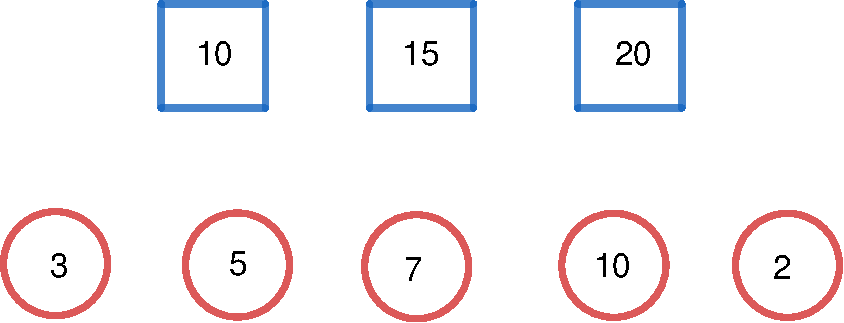
\includegraphics[width=0.9\textwidth]{img/ps1.pdf}
        \caption{Input graph $G$ where the blue vertices are the power stations and red vertices are the customers.}
        \label{fig:ps}
        \end{figure}
    \end{column}
    \pause
    \begin{column}{0.5\textwidth}
        \begin{figure}
        \centering
        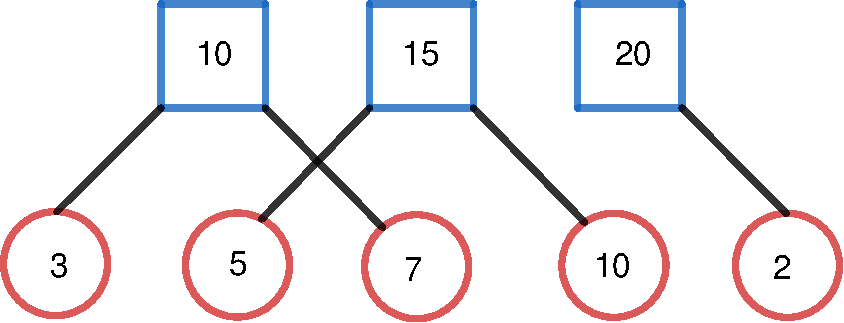
\includegraphics[width=0.9\textwidth]{img/ps2.pdf}
        \caption{A feasible solution to the POWER SUPPLY problem.\hfill \break}
        \label{fig:circle}
        \end{figure}
    \end{column}
\end{columns}

\begin{block}{Theorem (Ito et al.)}
The POWER SUPPLY problem is NP-complete \cite{DBLP:journals/tcs/ItoDHPSUU11}.
\end{block}
\end{frame}

\subsection{Power Supply Reconfiguration problem}
\begin{frame}{POWER SUPPLY RECONFIGURATION problem}
Suppose now that we are given two feasible solutions $s_0$ and $s_t$ of the POWER SUPPLY problem and are asked: \hfill \break 

Can one solution be transformed into the other by moving only one customer at a time and always remaining feasible?
\pause
\begin{columns}
    \begin{column}{0.5\textwidth}
        \begin{figure}
        \centering
        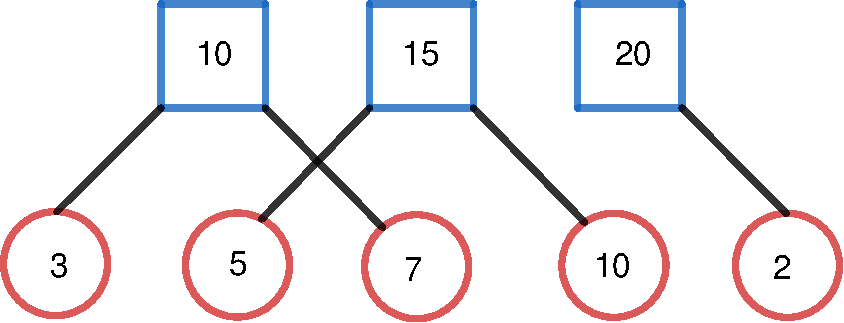
\includegraphics[width=0.9\textwidth]{img/ps2.pdf}
        \caption{Feasible solution $s_0$.}
        \label{fig:circle}
        \end{figure}
    \end{column}
    \begin{column}{0.5\textwidth}
        \begin{figure}
        \centering
        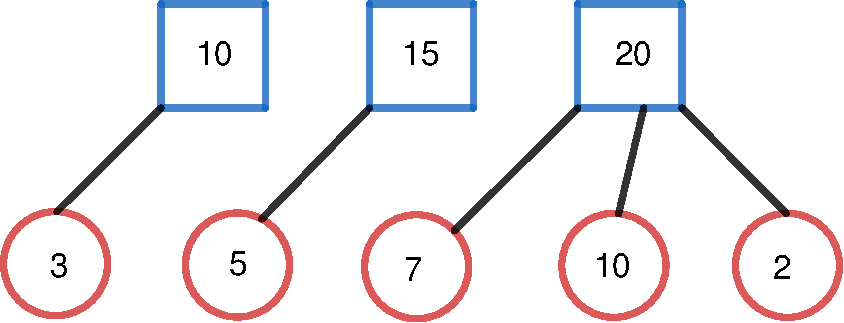
\includegraphics[width=0.9\textwidth]{img/ps4.pdf}
        \caption{Feasible solution $s_t$.}
        \label{fig:circle}
        \end{figure}
    \end{column}
\end{columns}
\end{frame}

\begin{frame}{POWER SUPPLY RECONFIGURATION problem}
\begin{columns}
    \begin{column}{0.3\textwidth}
        \begin{figure}
        \centering
        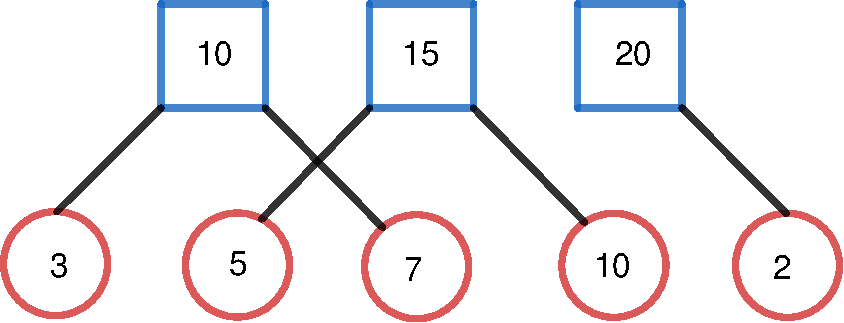
\includegraphics[width=1.1\textwidth]{img/ps2.pdf}
        \caption{Feasible solution $s_0$.\hfill \break \hfill \break \hfill \break \hfill \break}
        \label{fig:circle}
        \end{figure}
    \end{column}
    \begin{column}{0.3\textwidth}
        \begin{figure}
        \centering
        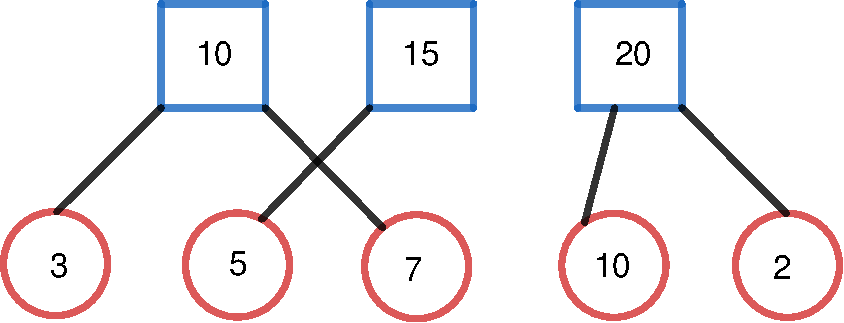
\includegraphics[width=1.1\textwidth]{img/ps3.pdf}
        \caption{Intermediate feasible solution $s_i$ where customer $10$ is moved.\hfill \break \hfill \break}
        \label{fig:circle}
        \end{figure}
    \end{column}
    \begin{column}{0.3\textwidth}
        \begin{figure}
        \centering
        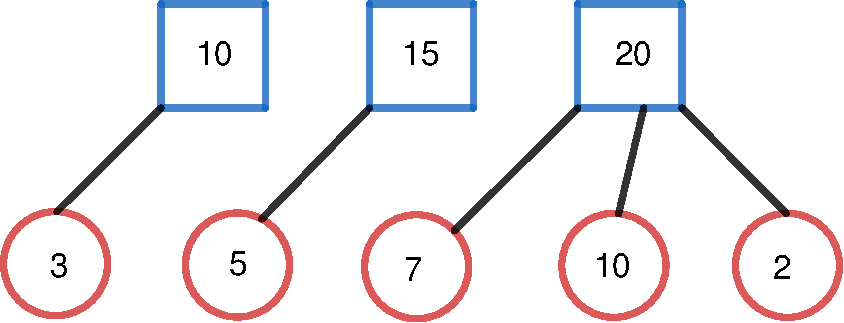
\includegraphics[width=1.1\textwidth]{img/ps4.pdf}
        \caption{Target feasible solution $s_t$ where customer $7$ is moved from previous intermediate solution.\hfill \break}
        \label{fig:circle}
        \end{figure}
    \end{column}
\end{columns}

    \begin{block}{Theorem (Ito et al.)}
    POWER SUPPLY RECONFIGURATION problem is PSPACE-complete \cite{DBLP:journals/tcs/ItoDHPSUU11}.
    \end{block}
\end{frame}

\section{Reconfiguration problems}
\subsection{Definition}
\begin{frame}{RECONFIGURATION problems}
  \begin{block}{Definition}
    Reconfiguration problems are computational problems in which we wish to find a step-by-step transformation between two feasible solutions of a problem such that all intermediate results are also feasible.
  \end{block}
\end{frame}


\begin{frame}{RECONFIGURATION problems}
    \begin{block}{Graph-theoric perspective}
    \begin{itemize}
        \item Reconfiguration graph where : 
        \begin{enumerate}
            \item The vertex set consists of all possible configurations (solutions).
            \item Two nodes are connected if the corresponding configurations can each be obtained from the other by the application of a single transformation rule, a \textit{reconfiguration step}.
        \end{enumerate}
        \item Any path or walk in the Reconfiguration graph $=$ \textit{Reconfiguration sequence}. 
    \end{itemize}
  \end{block}
\end{frame}

\section{Main themes}
\begin{frame}{RECONFIGURATION problems}
    \begin{block}{Main themes}
        \begin{enumerate}
            \item SATISFIABILITY RECONFIGURATION problems.
            \item SLIDING TOKENS problems. 
            \item SUBSET SUM RECONFIGURATION problems.
        \end{enumerate}
    \end{block}
\end{frame}




\subsection{SATISFIABILITY RECONFIGURATION}

\begin{frame}{SATISFIABILITY RECONFIGURATION}
    \begin{block}{satisfiability problem}
      The satisfiability problem, also called SAT is to test whether a CNF formula is satisfiable. An example of a CNF formula is $\varphi = (x_1 \vee x_2 \vee \neg x_3) \wedge (x_1 \vee \neg x_2 \vee x_3)$.
    \end{block}

    \begin{block}{Theorem (Cook-Levin)}
      SAT is NP-complete \cite{10.1145/800157.805047}.
    \end{block}

\end{frame}

\begin{frame}{SATISFIABILITY RECONFIGURATION}
    \begin{block}{SAT RECONFIGURATION problems}
       The solutions (satisfying assignments) of a given $n$-variable CNF $\varphi$ induce a subgraph $G(\varphi)$ of the $n$-dimensional hypercube, introducing two decision problems : 
       
       \begin{enumerate}
           \item Connectivity problem : Given a CNF formula $\varphi$, is $G(\varphi)$ connected?
           \item st-Connectivity problem : Given a CNF formula $\varphi$ and two solutions $s_0$ and $s_t$ of $\varphi$, is there a path from $s_0$ to $s_t$ in $G(\varphi)$?
       \end{enumerate}
    \end{block}
\end{frame}

\begin{frame}{SATISFIABILITY RECONFIGURATION}
    \begin{block}{Connectivity $\varphi = (x_1 \vee x_2 \vee \neg x_3) \wedge (x_1 \vee \neg x_2 \vee x_3)$. }
        \begin{columns}
            \begin{column}{0.5\textwidth}
                \begin{figure}
                \centering
                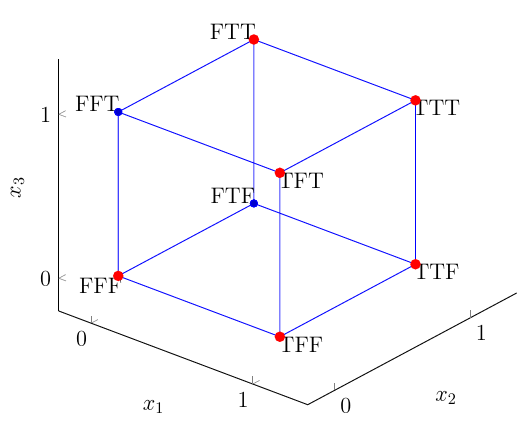
\includegraphics[width=0.9\textwidth]{img/sat_3.png}
                \caption{Reconfiguration graph of $\varphi$.}
                \label{fig:ps}
                \end{figure}
            \end{column}
            \pause
            \begin{column}{0.5\textwidth}
                \begin{figure}
                \centering
                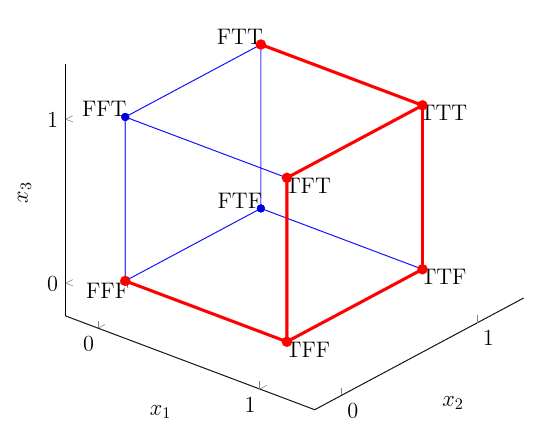
\includegraphics[width=0.9\textwidth]{img/sat_4.png}
                \caption{$G(\varphi)$.\hfill \break}
                \label{fig:circle}
                \end{figure}
            \end{column}
        \end{columns}
    \end{block}
\end{frame}

\begin{frame}{SATISFIABILITY RECONFIGURATION}
    \begin{block}{st-Connectivity $\varphi = (x_1 \vee x_2 \vee \neg x_3) \wedge (x_1 \vee \neg x_2 \vee x_3)$.}
        \begin{columns}
            \begin{column}{0.5\textwidth}
                \begin{figure}
                \centering
                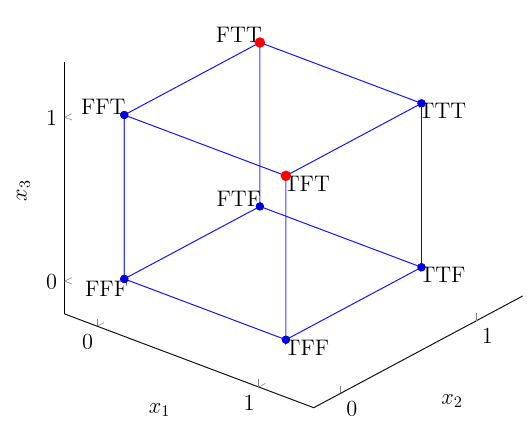
\includegraphics[width=0.9\textwidth]{img/sat_1.png}
                \caption{Reconfiguration graph of $\varphi$ with two satisfying assignments $s_0$ and $s_t$. }
                \label{fig:ps}
                \end{figure}
            \end{column}
            \pause
            \begin{column}{0.5\textwidth}
                \begin{figure}
                \centering
                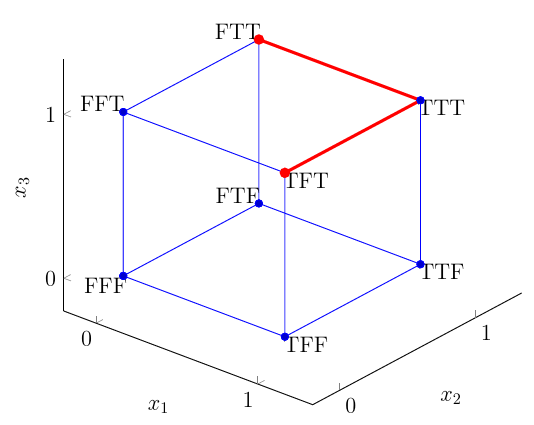
\includegraphics[width=0.9\textwidth]{img/sat_2.png}
                \caption{Reconfiguration sequence transforming $s_0$ to $s_t$. \hfill \break}
                \label{fig:circle}
                \end{figure}
            \end{column}
        \end{columns}
    \end{block}
\end{frame}

\begin{frame}{BOOLEAN SATISFIABILITY RECONFIGURATION}
    \begin{block}{Theorem (Gopalan et al.)}
    The Connectivity problem is PSPACE-complete \cite{gopalan_connectivity_2006}. 
    \end{block}

    \begin{block}{Theorem (Gopalan et al.)}
    The st-Connectivity problem is PSPACE-complete \cite{gopalan_connectivity_2006}. 
    \end{block}

\end{frame}


\subsection{SLIDING TOKENS RECONFIGURATION}

\begin{frame}{SLIDING TOKENS RECONFIGURATION}
\begin{block}{The SLIDING TOKENS problem} 
    \begin{flushleft}
      \textbf{Input Instance: } Two independent sets $I_1$ and $I_2$ of a graph $G = (V,E)$ s.t $|I_1| = |I_2|$ with a token placed on each vertex in $I_1$. \\
      \hfill \break
      \textbf{Question: } Is there a reconfiguration sequence from $I_1$ to $I_2$ ?\\
    \end{flushleft}
   \end{block}
   
   \begin{figure}
        \centering
        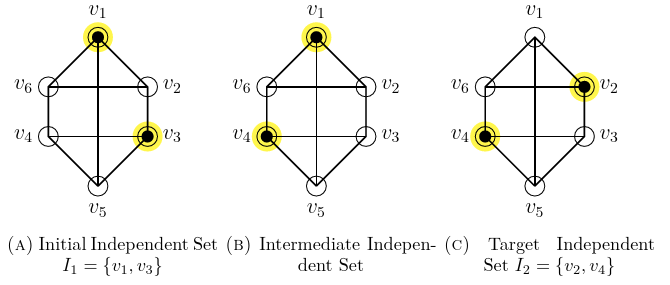
\includegraphics[scale=0.3]{img/sliding.png}
        \caption{Reconfiguration sequence from $I_1$ and $I_2$.}
        \label{fig:ps}
    \end{figure}
\end{frame}

\begin{frame}{SLIDING TOKENS RECONFIGURATION}
    
    Seen as the reconfiguration version of the Independent Set problem.
    
    \begin{block}{Theorem (E.Demaine \& R.Hearn)} The SLIDING TOKENS problem is PSPACE-complete \cite{hearn_demaine_ncl_book}. 
   \end{block}
\end{frame}

\begin{frame}{LABELLED SLIDING TOKENS}
    \begin{block}{The LABELLED SLIDING TOKENS problem}
        \begin{flushleft}
          \textbf{Input Instance: } Two independent sets $I_1$ and $I_2$ of a graph $G = (V,E)$ s.t $|I_1| = |I_2|$ with a labelled token placed on each each vertex in $I_1$ and each label is unique. \\
        \end{flushleft}
    \end{block}    
    
    \begin{block}{Theorem} The LABELLED SLIDING TOKENS problem is PSPACE-complete. 
   \end{block}
   
   \begin{proof} Reduction from the Nondeterministic Constraint Logic.
   \end{proof}
\end{frame}

\begin{frame}{Nondeterministic Constraint Logic}
    \begin{block}{Graph formulation}
    The computational model is a constraint graph $G = (V,E)$ \\ where :
     \begin{itemize}
        \item Each edge is assigned a weight. 
        \item Each vertex has a minimum inflow constraint.
        \item A configuration $=$ orientation of the edges. 
    \end{itemize}
    \end{block}
\end{frame}

\begin{frame}{Nondeterministic Constraint Logic}
  \begin{columns}
    \begin{column}{0.6\textwidth}
    \begin{block}{Restricted NCL}
    The constraint graph $G = (V, E)$
      \begin{itemize}
        \item $3$-regular.
        \item Uses only weights $\in \{1,2\}$ \\ 
        Red and blue edges.
        \item Uses only two types of vertices \\ 
        AND and OR vertices. 
        \item The minimum inflow constraint $ = 2$.
      \end{itemize}
   \end{block}
   \end{column}
   
   \begin{column}{0.4\textwidth}
       \begin{figure}
            \centering
            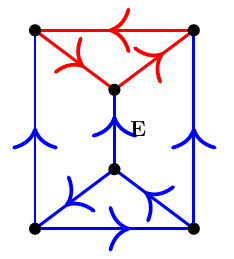
\includegraphics[scale=0.3]{img/restricted_ncl_1.png}
            \caption{Restricted NCL instance.}
            \label{fig:ps}
        \end{figure}
   \end{column}
   
\end{columns}   
\end{frame}

\begin{frame}{Nondeterministic Constraint Logic}
\begin{block}{Configuration-to-edge for Restricted NCL.}
    \begin{block}{Theorem (E.Demaine \& R.Hearn)}
    CONFIGURATION-TO-EDGE for restricted NCL is PSPACE-complete \cite{hearn_demaine_ncl_book}.
    \end{block}
        \begin{figure}
                \centering
                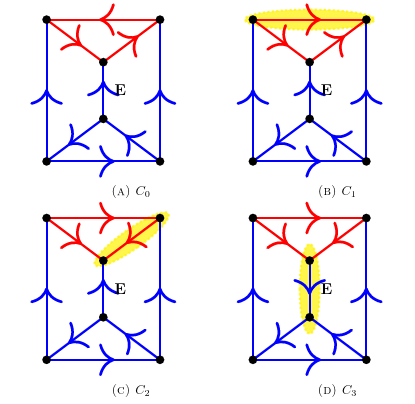
\includegraphics[scale=0.33]{img/restricted_ncl.png}
                \caption{Reconfiguration sequence reversing edge $E$.}
                \label{fig:ps}
        \end{figure}
    \end{block}

\end{frame}

\subsection{SUBSET SUM RECONFIGURATION}

\begin{frame}{SUBSET SUM RECONFIGURATION}
  \begin{block}{Subset Sum Problem}
      Given an integer $x$ and a set of integers $S = \{a_1, a_2, \dots, a_n\}$, we wish 
      to find a subset $A \subseteq [n]$ such that $\sum_{i \in A} a_{i} = x.$
  \end{block}
   \begin{block}{SUBSET SUM RECONFIGURATION}
    Two variants : 
      \begin{enumerate}
          \setlength\itemsep{1em}
          \item Add/remove $y$, keep sum in target range. \\
          ({\footnotesize considered by Ito and Demaine, referred as SUBSET SUM RECONFIGURATION problem (SSR).}) \\ 
          
          \item Swap $y, z$ and $y + z$, keep target sum. \\
          ({\footnotesize considered by Cardinal et al., referred as $k$-move SUBSET SUM RECONFIGURATION problem ($k$-move SSR).}) 
      \end{enumerate}
    \end{block}

\end{frame}

\begin{frame}{SUBSET SUM RECONFIGURATION}
  \begin{columns}
        \begin{column}{0.5\textwidth}
            \begin{figure}
                \centering
                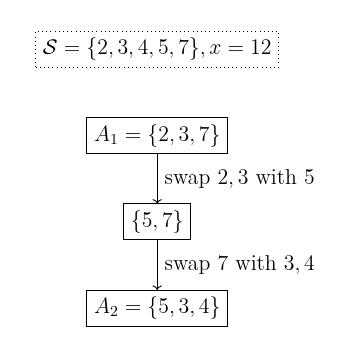
\includegraphics[width=0.9\textwidth]{img/s_1.png}
                \caption{An instance of the $k$-move SSR problem where $k = 3$.}
                \label{fig:ps}
            \end{figure}
        \end{column}
        \pause
        \begin{column}{0.5\textwidth}
            \begin{figure}
                \centering
                 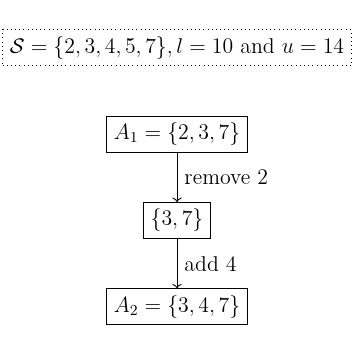
\includegraphics[width=0.9\textwidth]{img/s_2.png}
                \caption{An instance of the SSR problem.\hfill \break}
                \label{fig:circle}
            \end{figure}
        \end{column}
    \end{columns}
\end{frame}


\begin{frame}{SUBSET SUM RECONFIGURATION}
   \begin{block}{Theorem (Ito et al.)}
   The SUBSET SUM RECONFIGURATION problem is NP-hard \cite{Ito11approximabilityof}.
   \end{block}
  
   \begin{block}{Theorem (Cardinal et al.)}
   The $k$-move SUBSET SUM RECONFIGURATION Problem is PSPACE-complete for $k = 3$ \cite{cardinal_reconfiguration_2018}.
   \end{block}
\end{frame}


\begin{frame}{Geometric interpretations}
    \begin{block}{Constrained Hypercube Path problem} Given two vertices $s, t$ of the $n$-hypercube, both contained in a polytope
    $P := \{x \in \mathbb{R}^n : Ax \leq b\}$ for some $A = (a_{ij}) \in \mathbb{Z}^{d \times n}$ and $b \in \mathbb{Z}^d$, does there exist a path from $s$ to $t$ in the hypercube, all vertices of which lie in $P$?
    \end{block}
\end{frame}

\begin{frame}{Geometric interpretations}
   \begin{block}{SSR problem $\rightarrow$ Constrained hypercube path}
       \begin{itemize}
           \item Let $x \subseteq \{0,1\}^n$ Boolean variable indicating if an item is chosen or not. 
           \item The solution space of an instance of the SSR problem is represented by an $n$-hypercube. 
           \item The solutions to this given instance are the points of the $n$-hypercube that lie in the polytope $P := \{k \leq \sum_{i=1}^{n} x_{i}w_{i} \leq c\}$.
           \item The SSR problem is equivalent to the 
           Constrained Hypercube path problem where $d = 2$ since it involves exactly two linear constraints. 
           
       \end{itemize}
   \end{block}
\end{frame}

\begin{frame}{Geometric interpretation}
  \begin{block}{Example : SSR input instance}
  \begin{itemize}
      \item $\mathcal{S} = \{1,3,6\}$.
      \item The lower bound $= 1$. 
      \item The upper bound $ = 7.$
      \item $A_1 = \{6\}$ and $A_2 = \{1,3\}.$
  \end{itemize}
  \end{block}
\end{frame}


\begin{frame}{Geometric interpretation}
  \begin{block}{SSR instance $\rightarrow$ Constrained Hypercube path problem.}
    \begin{columns}
        \begin{column}{0.5\textwidth}
            \begin{figure}
            \centering
            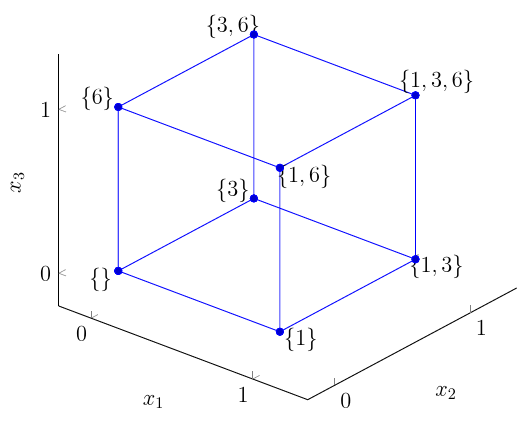
\includegraphics[width=0.9\textwidth]{img/subset_1.png}
            \caption{$n$-hypercube induced by all possible configurations of the given input SSR instance.}
            \label{fig:ps}
            \end{figure}
        \end{column}
        \pause
    \begin{column}{0.5\textwidth}
        \begin{figure}
        \centering
        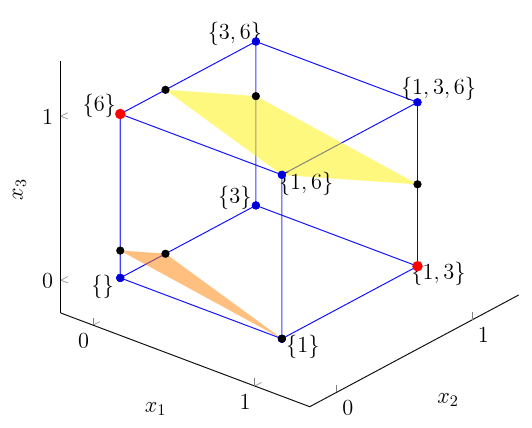
\includegraphics[width=0.9\textwidth]{img/subset_2.png}
        \caption{Polytope defined by the two linear constraints of the SSR problem.\hfill \break}
        \label{fig:circle}
        \end{figure}
    \end{column}
\end{columns}
 \end{block}
\end{frame}

\begin{frame}{Geometric interpretations}
  \begin{block}{SSR instance $\rightarrow$ Constrained Hypercube path problem.}
            \begin{columns}
                \begin{column}{0.5\textwidth}
                    \begin{figure}
                    \centering
                    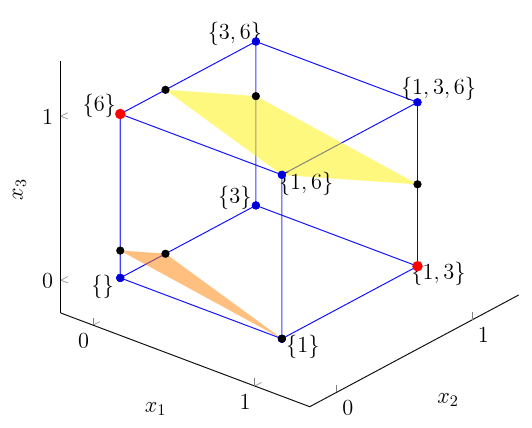
\includegraphics[width=0.9\textwidth]{img/subset_2.png}
                    \caption{Polytope defined by the two linear constraints of the SSR problem.}
                    \label{fig:ps}
                    \end{figure}
                \end{column}
                \begin{column}{0.5\textwidth}
                    \begin{figure}
                    \centering
                    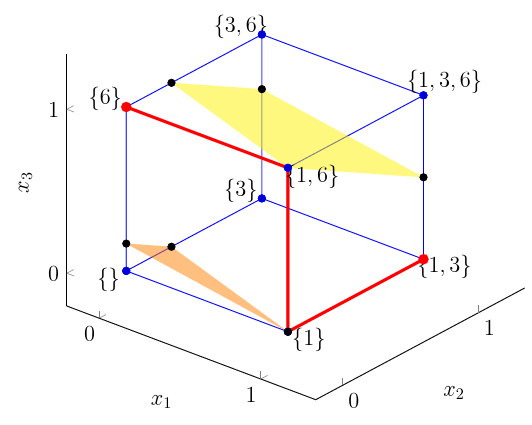
\includegraphics[width=0.9\textwidth]{img/subset_3.png}
                    \caption{Reconfiguration sequence $S$ transforming $A_1$ to $A_2$ while satisfying the capacity and treshold constraint.\hfill \break}
                    \label{fig:circle}
                    \end{figure}
                \end{column}
            \end{columns}
  \end{block}
\end{frame}

\begin{frame}{Geometric interpretations}
   \begin{block}{$k$-move SSR $\rightarrow$ Constrained hypercube path}
       \begin{itemize}
            \item Let $x \subseteq \{0,1\}^n$ Boolean variable indicating if an integer is chosen or not. 
           \item The solution space of a $k$-move SSR instance is represented by $H_n^{k}[Q]$ which is the $kth$ power of the $n$-hypercube $Q$ where two vertices are connected iff their symmetric difference is at most $k$. 
           \item The solutions to this given instance are the points of the  $H_n^{k}[Q]$ that lie in the polytope $P := \{ \sum_{i=1}^{n} x_{i}a_{i} = x\}$.
           \item The $k$-move SSR is equivalent to the Constrained Hypercube path problem where $d = 1$ since it involves exactly one linear constraint. 
       \end{itemize}
   \end{block}
\end{frame}


\begin{frame}{Geometric interpretation}
  \begin{block}{Example : $3$-move SSR input instance}
  \begin{itemize}
      \item $\mathcal{S} = \{2,3,5\}$.
      \item Target sum $x = 5.$
      \item $A_1 = \{5\}$ and $A_2 = \{2,3\}.$
  \end{itemize}
  \end{block}
\end{frame}


\begin{frame}{Geometric interpretations}
  \begin{block}{$3$-move SSR instance $\rightarrow$ Constrained Hypercube path problem.}
            \begin{columns}
                \begin{column}{0.5\textwidth}
                    \begin{figure}
                    \centering
                    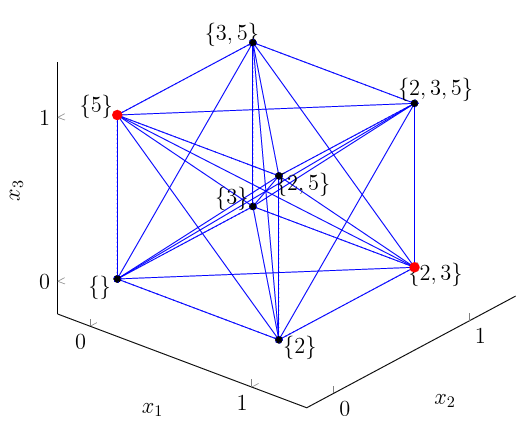
\includegraphics[width=0.9\textwidth]{img/3SSR_1.png}
                    \caption{$H_3^{3}[Q]$.}
                    \label{fig:ps}
                    \end{figure}
                \end{column}
                \begin{column}{0.5\textwidth}
                    \begin{figure}
                    \centering
                    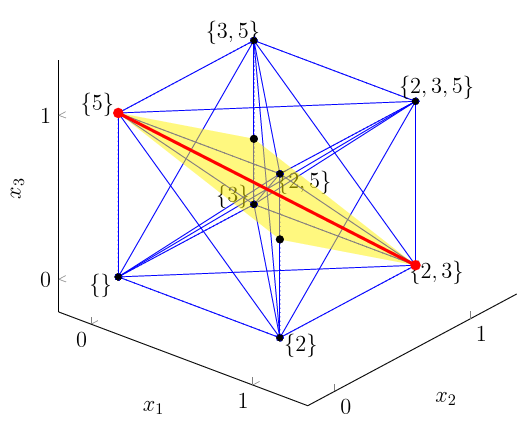
\includegraphics[width=0.9\textwidth]{img/3SSR_2.png}
                    \caption{Reconfiguration sequence $S$ transforming $A_1$ to $A_2$ while satisfying the target sum constraint.\hfill \break}
                    \label{fig:circle}
                    \end{figure}
                \end{column}
            \end{columns}
  \end{block}
\end{frame}


\section{Open questions}

\begin{frame}{Open questions}
    \begin{block}{SSR} Given an SSR instance, is the subgraph induced by all the feasible solutions connected ? 
    \end{block}
    \begin{columns}
        \begin{column}{0.5\textwidth}
            \begin{figure}
                \centering
                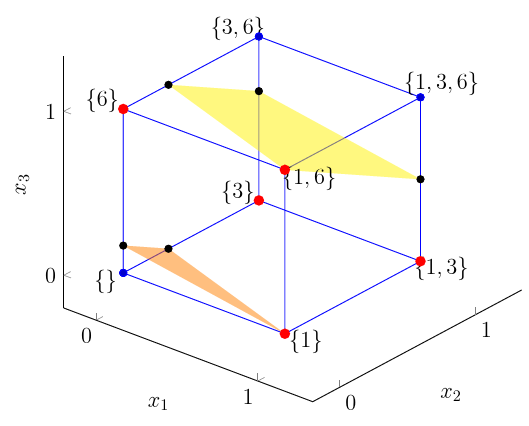
\includegraphics[width=0.9\textwidth]{img/subset_conn_4.png}
                \label{fig:ps}
            \end{figure}
        \end{column}
        \begin{column}{0.5\textwidth}
            \begin{figure}
                \centering
                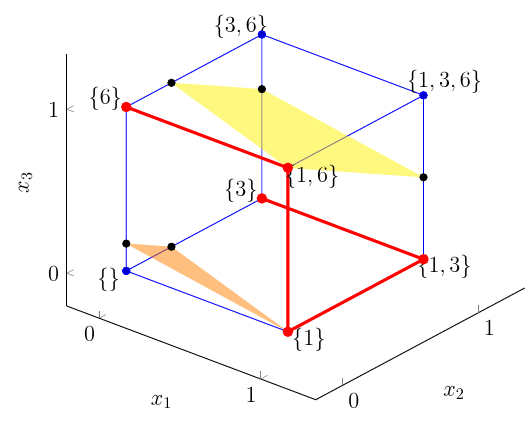
\includegraphics[width=0.9\textwidth]{img/subset_conn_5.png}
                \label{fig:circle}
            \end{figure}
        \end{column}
    \end{columns}
\end{frame}


\begin{frame}{Open questions}
    \begin{block}{$k$-move SSR} Given a $k$-move SSR, is the subgraph induced by all the feasible solutions connected ? 
    \end{block}
\end{frame}

\begin{frame}[allowframebreaks]{References}
   \printbibliography    
\end{frame}

\thanksframe{Thank you for your attention. \\}


\end{document}
